\section{Aerodynamic concept analysis}
\label{ch:aero_analysis}
In order to analyse the aerodynamic characteristics of the proposed concepts a software tool was developed. This chapter will deal with the development and implementation of this program. First section \ref{subsec:aerotool} will discuss the tool development process. Secondly section \ref{subsec:appaeroanal} 

\subsection{Development of aerodynamic analysis tool}
\label{subsec:aerotool}
For analysing the aerodynamic characteristics of each concept the modified Newtonian method will be used. This method relates the inclination angle $\gls{sym:chi}$ of a flat plate with respect to an incoming flow to the magnitude of its coefficient of pressure, as shown in equation \ref{eq:modnewtonian} \cite{AndersonJr.2006}.
\begin{multicols}{2}
\begin{equation}
\gls{sym:CP}=\gls{sym:CP}_{max}sin^{2}(\gls{sym:chi})
\label{eq:modnewtonian}
\end{equation} \break
\begin{equation}
\gls{sym:CP}_{max}=\frac{p_{O_{2}}-p_{\infty}}{\frac{1}{2}\rho_{\infty}V_{\infty}^{2}}
\label{eq:cpmax}
\end{equation}
\end{multicols}
In equation \ref{eq:modnewtonian} $\gls{sym:CP}_{max}$ is the value of $\gls{sym:CP}$ in the stagnation point of an arbitrary body. Since the stagnation point is per definition located behind a normal shock its value can be found from the normal shock relations. The result of doing this is shown in equation \ref{eq:cpmax}. Here $p_{O_{2}}$ denotes the total pressure in the stagnation point and can be found using equation \ref{eq:po2} \cite{AndersonJr.2007}.

\begin{equation}
\frac{p_{O_{2}}}{p_{\infty}}=\left(\frac{(\gls{sym:gamma}+1)^{2}M_{\infty}^{2}}{4\gls{sym:gamma} M_{\infty}^{2}-2(\gls{sym:gamma}-1)}\right)^{\frac{\gls{sym:gamma}}{\gls{sym:gamma}-1}}\left(\frac{1-\gls{sym:gamma}+2\gls{sym:gamma} M_{\infty}^{2}}{\gls{sym:gamma}+1}\right)
\label{eq:po2}
\end{equation}

Furthermore it can be noted that $\frac{1}{2}\rho_{\infty}V_{\infty}^{2}=\frac{\gls{sym:gamma}}{2}p_{\infty}M_{\infty}^{2}$ \cite{AndersonJr.2007}. Combining this with equation \ref{eq:cpmax} produces equation \ref{eq:cpmaxfinal}, where the ratio $\frac{p_{O_{2}}}{p_{\infty}}$ can be calculated using equation \ref{eq:po2}.

\begin{equation}
C_{p_{max}}=\frac{2}{\gls{sym:gamma} M_{\infty}^{2}}\left(\frac{p_{O_{2}}}{p_{\infty}}-1\right)
\label{eq:cpmaxfinal}
\end{equation}

By dividing the surface of the body to be analysed into many triangular elements the pressure coefficient distribution of said body can be determined numerically. A velocity magnitude is given as input, together with the angle of attack \gls{sym:alpha} and sideslip angle \gls{sym:beta}. Following this the outward surface normal vector is computed in Cartesian coordinates for every element, after which the velocity unit vector is computed with equation \ref{eq:unitV}. To determine $sin(\gls{sym:chi})$ for every element the dot product of the velocity unit vector with the surface normal vector is then taken, as shown in equation \ref{eq:dotproduct}.
\begin{multicols}{2}
\begin{equation}
\gls{sym:Vhat}=\frac{\gls{sym:Vv}}{\gls{sym:V}}
\label{eq:unitV}
\end{equation} \break
\begin{equation}
sin(\gls{sym:chi})=\gls{sym:Vhat} \bullet \hat{n}
\label{eq:dotproduct}
\end{equation}
\end{multicols}
Using $C_{p_{max}}$ and $sin(\gls{sym:chi})$ the \gls{sym:CP} for every surface element is calculated, after which it is multiplied with the element area and the element surface normal vector. This results in an elemental pressure force in three dimensions from which the lift and drag forces can be determined. By then summing the resultant forces for all elements the total body forces are found. Next to the body forces the resultant aerodynamic moment can also be found. For this the location of the \acrfull{cg} is used as input, after which the moments about the \gls{cg} caused by the force on each element can be summed. 

In addition to determining the aerodynamic forces and moments acting on the body, the heat flux in the stagnation point is also computed. A generalized equation to predict the heat flux on a body can be found in \cite{AndersonJr.2006,Tauber1986}. This equation is shown in \ref{eq:heatflux}.
\begin{equation}
q_{w}=\rho_{\infty}^{N}V_{\infty}^{M}C
\label{eq:heatflux}
\end{equation}

In the stagnation point it is furthermore known that: 
\begin{multicols}{2}
\begin{equation}
\label{eq:stagdens}
N=0.5
\end{equation} \break
\begin{equation}
\label{eq:stagspeed}
M=3.0
\end{equation}
\end{multicols}
\begin{equation}
\label{eq:stagcoefficient}
C=1.83 \times 10^{-8} R^{-\frac{1}{2}}\left(1-\frac{h_{w}}{h_{0}}\right)
\end{equation}
Where in equation \ref{eq:stagcoefficient} $R$ denotes the local body radius in the stagnation point and $h_{w}$ and $h_{0}$ comprise of the wall and total enthalpies respectively. An additional assumption that is made here is that $\frac{h_{w}}{h_{0}}\ll 1$. Justification for this statement can be found in the fact that the wall temperature must be smaller than the melting or decomposition temperature during the entire flight. Thus, although the temperature can become very high, the resulting wall enthalpy $h_{w}$ will still be much smaller than the total enthalpy $h_{0}$ \cite[p.347]{AndersonJr.2006}. %In addition to this the computed heat flux will increase as a result of neglecting this factor. One can see that if in later design phases the enthalpy ratio is included into the calculations this will relax the design constraints.
Combining equations \ref{eq:heatflux}, \ref{eq:stagdens}, \ref{eq:stagspeed}, \ref{eq:stagcoefficient} into one single equation produces:
\begin{equation}
q_{w_{stagnation}}=1.83 \times 10^{-8}\rho_{\infty}^{0.5} V_{\infty}^{3.0} R^{-\frac{1}{2}}
\label{eq:qstag}
\end{equation}
Where $q_{w_{stagnation}}$ denotes the heat flux into the body at the stagnation point. This will be used as input for the thermodynamic model in order to compute the required thicknesses of the \acrfull{tps} lay-up.

\subsection{Model verification \& validation}
\label{subsec:aeroverval}
After the model construction verification was carried out to determine whether the model correctly implemented the calculations of the modified Newtonian method. This was done by placing two triangular surface elements in a flow. First at an angle and secondly normal to the flow. The model outputs were verified by also calculating the results by hand.

Following the verification process the model was validated using experimental values of different parameters. Each separate validation case will be treated here.

\subsubsection{\gls{sym:CD}-validation against experimental hypersonic drag of a sphere}
For the first model validation case a comparison was made the between the \gls{sym:CD}-value of a sphere in hypersonic flow that were computed by the model and as found in an experiment. It was found that for hypersonic Mach numbers the experimental \gls{sym:CD}-value of a sphere is $0.92$ \cite{Bailey1966,AndersonJr.2007,Cox1965}. When computing \gls{sym:CD} numerically with the modified Newtonian method using $>10,000$ surface elements produces $\gls{sym:CD}=0.916$, which coincides with a discrepancy of $0.5\%$ of the experimental value.

\subsubsection{Element \gls{sym:CP}-validation against experimental hypersonic drag of a cone cylinder}


%\begin{figure}[h]
%	\centering
%	\begin{subfigure}[b]{0.49\textwidth}
%		\centering
%		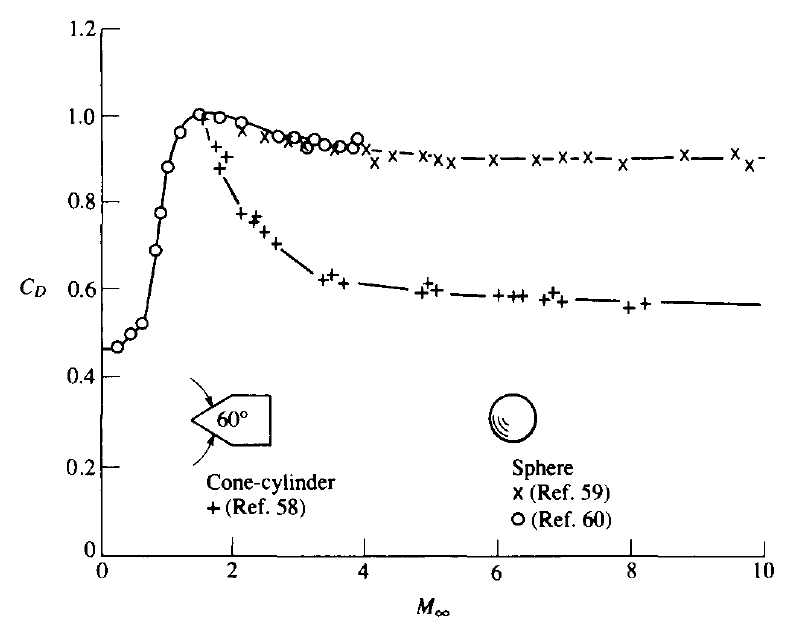
\includegraphics[width=0.95\textwidth]{./Figure/CD_sphere_exp}
%		\caption[Variation of measured \gls{sym:CD} with Mach number for a sphere and cone-cylinder]{Variation of measured \gls{sym:CD} with Mach number for a sphere and cone-cylinder \cite{AndersonJr.2007,Cox1965}}
%		\label{fig:exp_cd}
%	\end{subfigure}
%	\begin{subfigure}[b]{0.49\textwidth}
%		\centering
%		
\includegraphics[width=0.95\textwidth]{./Figure/Nyan}
%		\caption{heading}
%		\label{fig:num_cd}
%	\end{subfigure}
%	\caption{Comparison of experimental and numerical \gls{sym:CD}-values}
%	\label{fig:comparison_cd}
%\end{figure}

\subsection{Application of analysis tool to system concepts}
\label{subsec:appaeroanal}
After the model development 